\documentclass{llncs}

\usepackage{makeidx}  % allows for indexgeneration

\usepackage{graphics, graphicx, xcolor}

%\usepackage{times}

\newcommand{\authcmt}[2]{\textcolor{#1}{#2}}
\newcommand{\yuncong}[1]{\authcmt{red}{[YC: #1]}}
\newcommand{\yoav}[1]{\authcmt{blue}{[YF: #1]}}

\begin{document}
%
%\mainmatter              % start of the contributions
%
\title{Robust Landmark Detection for Alignment of Mouse Brain Section Images}
%
\titlerunning{Robust Landmark Detection for Mouse Brain Images}  % abbreviated title (for running head)
%                                     also used for the TOC unless
%                                     \toctitle is used
%
\author{Yuncong Chen, David Kleinfeld, Martyn Goulding \and Yoav Freund}
%
\authorrunning{Yuncong Chen et al.} % abbreviated author list (for running head)
%
%%%% list of authors for the TOC (use if author list has to be modified)
% \tocauthor{Yuncong Chen, Yoav Freund}
%
\institute{Department of Computer Science and Engineering, \\University of California, San Diego, La Jolla, CA 92122, USA}




\maketitle              % typeset the title of the contribution

\begin{abstract}

Brightfield and fluorescent imaging of whole brain sections is a fundamental tool in anatomical studies on brain functions. As automation of the sectioning and image acquisition processes become more efficient, there is an increasing need to automate the post-processing of sections for alignment and three dimensional visualization. There is a further need to facilitate the development of a ``digital atlas", i.e. a brain-wide map annotated with cell type, tract tracing and physiological data, which serves as the underpinning of circuits analysis as well as for quantitative analysis of phenotypical variation. Currently, such maps are created by hand.

In this work we describe the first steps in developing a semi-automated system to construct a mouse brain atlas that combines annotation, registration and atlas building in an iterative framework. This atlas stores landmark models, uses them to detect landmarks from new images and maps the images onto the atlas's standardized coordinate system; meanwhile, the models in the atlas are updated based on newly registered images.

The aspect of the project described here is a semi-supervised learning
system for identifying landmarks. It detects and models regions with distinct texture that are consistent across sections. It also identifies boundary segments for regions that are not compact. Experiments show that the detected landmarks correspond well with labellings by experienced anatomists. The results serve as a promising basis for the next stage of registration and atlas building.


\iffalse
Brightfield and fluorescent imaging of whole brain sections is a fundamental tool in anatomical studies on brain functions. 
Current technology allows a whole brain to be scanned in a matter of hours. At the same time, there is an increasing number of fluorescent markers that can be used to label neurons with specific
phenotypes. As the number of available images mounts, the manual work
required to analyze these images becomes a major bottleneck and automated tools that aggregate information in the images become necessary.

In this work we describe the first steps in a project whose goal is to build an ``active" atlas, which combines annotation, registration and atlas building in a semi-automated iterative framework. This atlas explicitly models region landmarks, uses these models to detect landmarks from new images for registration; meanwhile, the models are updated based on newly registered images. 

The part of the project described here is a semi-supervised learning
system for identifying region landmarks. It detects and models regions that have distinct texture and are consistent across sections. It also models stable boundary segments. Experiments show that the detected landmarks correspond well with labellings by experienced anatomists. The results serve as a promising basis for the next stage of registration and atlas building.
\fi

\iffalse
Brightfield and flurescent imaging is of central importance in mouse brain
studies. As automation is improving, a whole brain can be imaged in 
one hour. At the same time, there is an increasing number of
fluorescent markers that can be used to identify neurons with specific
phenotypes. As the number of available images mounts, the manual work
required to analyze these images becomes a major bottleneck and 
automated tools for processing those images become necessary.

In this work we describe the first steps in a project whose goal is to
create a ``digital atlas'' of the brain. A digital atlas in this
context is computer software (and data) that takes as input a stack of
section images and maps those images onto a standarized coordinate
system for the mouse brain. Such mapping is a prerquisite for
automatic quantitative analysis of phenotypical variation. Currently
such mapping is done manually.

The part of the project described here is a semi-supervised learning
system for identifying landmarks in brain slice images. The
identification of such landmarks is based on identifying regions with
distinct texture and the boundaries between these landmarks. Thew
digital atlas will be compiled by comparing different brains and
identifying the consistent landmarks.
\fi

\keywords{landmark detection, atlas building, mouse brain, registration, automated annotation}

\end{abstract}
%

\section{Introduction}

Brightfield and fluorescent imaging is a fundamental tool in mouse brain studies. As sectioning and image acquisition becomes more efficient, there is an increasing need to automate the post-processing of sections for alignment and three dimensional visualization. There is also a need to facilitate the development of standardized atlases. A standardized atlas maps image series of different specimens to a common coordinate system, and shows a brain-wide map annotated with information such as cell type, tract tracing and physiological data. Such map serves as the underpinning of circuits analysis as well as quantitative analysis of phenotypical variation.

%On the one hand, this allows the new specimen to be compared with annotations and cell type maps collected from previous specimens; on the other hand, new specimens augment the atlas by introducing annotations for new structures or by providing additional cell type data demonstrated by new markers.

The Allen Mouse Brain Atlas is constructed by registering sections of a single brain.

 While it is useful as a visual guide for annotating new images by hand, there is no easy solution for aligning new image series to the atlas. Software for registration usually requires heavy human intervention, such as picking the landmarks or adjusting parameters that lack intuitive meaning.


Update itself. 


A fixed atlas is not optimal, as new 

building an atlas automatically 

Several functions can be enabled by modeling the annotated regions. First, the regions can serve as landmarks in registration. Compared to point landmarks they can have more expressive features such as texture and shape. Second, the 


In order to do this, we need to model the landmarks. 

We propose building an ``active" atlas. In such an atlas, characteristics of annotated regions are modelled using machine learning. These models are then used to detect similar regions in new images. Detected regions serve as landmarks for both intra-specimen registration and specimen-atlas registration. Once the new images are aligned to the atlas, region models are updated based on characteristics of detected regions in the aligned new images. Essentially, the atlas ``actively" adapts to registered specimens, and ``actively" annotates new specimens for easier registration. In contrast to most existing work that either focuses on building an atlas by registering a single image series, or on aligning image series to an fixed atlas, the active atlas combines annotation, registration and atlas building into an iterative framework that is particularly suitable for processing a large number of specimens in an incremental fashion.

% and with as little human supervision as possible

One crucial component in building an active atlas is identifying the landmarks. Until the region models are trained with sufficiently many examples, the system must obtain the annotation in other ways. Having human labellers do the annotation is time-consuming. In this paper, we propose an automatic approach.

Our particular study focuses on the brainstem. Unlike the cerebrum and the cerebellum, where neurons form high-contrast layered structures such as the cortex, the brainstem mostly contains nuclei, which are compact clusters of neurons. For example, Figure 1 shows the facial motor nucleus. Neurons in each nucleus have similar size, shape and stain sensitivity, often also demonstrating uniform density and particular directionality. This gives each nuclei a distinctive texture, allowing them to be robustly identified when building the atlas. The fact that they are well localized also makes them perfect landmarks for registration. In addition to nuclei, fiber tracts are also recognizable structures in the brainstem. In particular, the directionality of a tract serves as an important feature of the landmark.

We therefore aim to model the landmarks based on texture. Section 3 describes how we represent textures using Gabor filters and superpixels. Section 4 explains how we identify potential landmark regions based on texture distinctiveness. Section 6 describes how we detect stable boundary segments based on regions to improve robustness. Section 7 describes how landmarks are matched between sections.

%Allen Reference Atlas has limited details on the brainstem, which is also one of our motivations for building a new atlas.
%
%New landmarks that do not exist in previous specimens, 
%
%variation information used for identifying consistent landmarks

\section{Related Work}

\begin{description}

\item{Intensity based Registration}
Mostly intensity based


\item{Point Landmark Detection}

SIFT

\item{Saliency and Objectness Detection}

global rarity scheme

center-surround scheme

\yoav{Is there work that uses notion of statistical significance in
  this context?}

\item{Texture Representation}

gabor filter

textons


\end{description}

\section{Representing Texture using Histograms of Gabor Textons} 

Images in the stack are filtered using Gabor filters with nine orientations and ten scales. From each image, 1000 feature vectors are sampled. We reduce the data by quantizing these 99 dimensional feature vectors using K-Means. First, 100 clusters are generated; then clusters with close centroids are merged. The final cluster centroids are the textons. 

%\begin{figure}
%\caption{Gabor Filters}
%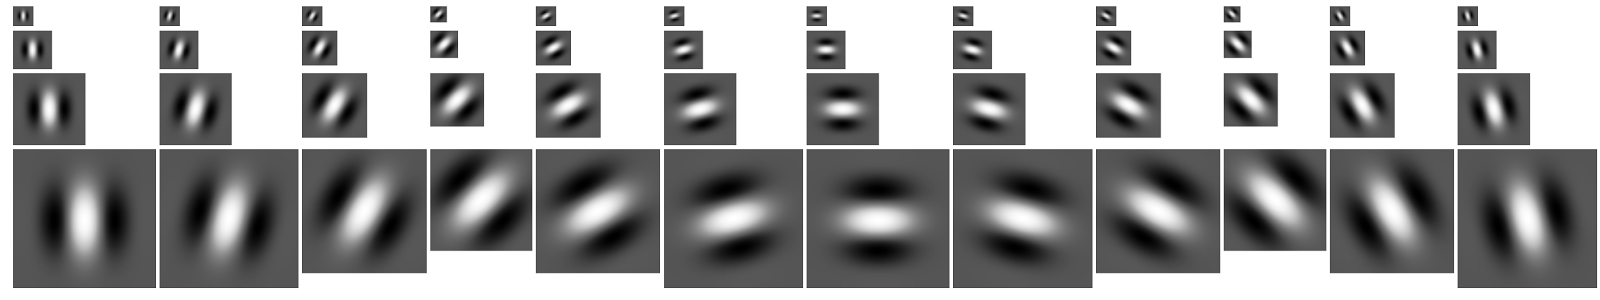
\includegraphics[width=0.5\textwidth]{../figures/gabor}
%\end{figure}

We further reduce the data by describing texture at the level of superpixels. For each superpixel, texture is represented by the histogram of the textons it contains. The superpixels are obtained using the SLIC algorithm. 

Since different sections may be oriented at different angles, and in order for two identical but slightly rotated textures to match, we need the features to be rotation-invariant. To this end, we compute the energy distribution over orientations for each feature vector, and shift all feature vectors such that the modes of directional energy distributions are aligned. In this way, the texture is decoupled from directionality. Note that the directionality is still useful, particularly for describing fiber tracts.

\section{Evaluating Region Significance using Statistical Test}

Now that textures are represented using histograms of Gabor textons, we need to find regions with distinct texture. In this section, we propose a score that measures the significance of a region. In the next section, we describe a method for finding potential regions as sets of connected superpixels. 

The significance score of a region is a linear combination of three terms. 

The first factor is the distinctiveness of this region's texture, or in other words, how different its texture is from the surrounds. Since textures are represented as histograms, this problem naturally leads to a statistical test on whether the region's average texton histogram and those of its surrounds are sampled from the same distribution. In our experiment, the chi-squared test is used. The p-value of this test can be used as a quantitative measure of the distinctiveness. Since a region often has many neighbouring regions with different textures, the test is made between the region's histogram and that of every surrounding superpixel, and the largest p-value is used. 

The second factor is the texture homogeneity within the region. This is defined in terms of the mean dissimilarity between all superpixels in the region and the region average.

The third factor stems from the fact that most nuclei have compact shapes. A common measure for the compactness of a closed curve is the isoperimetric quotient, defined as the square of the circumference divided by the enclosing area. We use the number of superpixels in the region as a proxy for the area and the number of surrounding superpixels as that for the circumference.

\section{Finding Significant Regions with Region Growing and Clustering}

Region growing is performed on every superpixel. Starting from a singleton containing the seed superpixel, the greedy procedure considers all neighbours of the current set, and iteratively adds the one whose texton histogram is closest to the current region histogram. The growing stops when the region reaches 10\% of the total area. Eventually, the region at the point when the significance score is the largest is returned. Figure x shows examples of this procedure.

%The termination criteria is a threshold on the histogram dissimilarity between the newly added superpixel and the set average. Instead of using a pre-determined threshold, we over-grow the region until its size reaches 10\% of the total area, and record this dissimilarity at every iteration. The dissimilarity would be the largest when the growing incorporates a superpixel that is the most different in hindsight, and thus the region just before this point is returned as the result of growing. This maximum dissimilarity can be used as a measure for the contrast, since every added superpixel is lower than this value.

We call the set of superpixels that grows from a seed the \textit{expansion region} of the seed. If a region has distinct texture, the expansion regions grown from the superpixels inside this region are expected to be almost identical, and they will have no overlap with the expansion regions from superpixels outside of this region (see Figure x). In other words, the expansion regions form clusters. The denser a cluster is, the more significant the region it represents. Using Jaccard index as the pairwise distance, we group the expansion regions using hierarchical clustering. We then find the groups whose size is large enough, and select the expansion region with the highest significance score as the representative of that group.

Finally, the representative expansion regions from all groups are ranked according to the significance scores. Figure x shows the top 10 regions.

How to model the regions...

%\section{Human Supervision}
%
%\yoav{Describe how salient region detection improves efficiency of human labeling.}
 
\section{Evaluating Boundary Robustness by Region Consensus}

In addition to compact-shaped regions, boundaries between structures are also useful landmarks. In many cases, nuclei are separate from each other and have clear closed contours. In other cases, a region has a clear boundary on one side, but on the other side is a gradual transition into the neighboring texture. One example is shown in Figure x. For these regions only partial boundary can be identified.

As region growing is sensitive to the seed, the expansion regions from different seeds in the same anatomical structure are not always consistent. However, most of them will agree on parts of the boundary that are stable (see Figure x). This motivates a region consensus approach for identifying the robust boundary segments.

%Compared to modelling a complete contour, one additional benefit of modelling boundary segments, is that different sides of a region can be assigned different significance scores.

The strategy is to let each expansion region vote for every of its boundary segment. The weight of the vote cast to a particular segment depends on the chi-squared distance between the region average and the superpixel at the other side of the segment. The boundariness score for a segment $(i,j)$ is:

$$
b((i,j)) = \sum_{i: j\in \delta S_i} \frac{d(\bar{h}_i, h_j)}{|S_i|}
$$

We also record the set of superpixels that vote for a segment, and call it the \textit{supporter set} of the segment.

We discard boundary segments whose vote is lower than a threshold and model the remaining segments. Instead of modelling individual segments separately, we want to group segments that receive votes from the same group of expansion regions. Therefore we define the association between two boundary segments to be the Jaccard index of their supporter sets, and apply hierarchical clustering to obtain boundary segment groups. Each group represents a partial boundary. All partial boundaries are ranked according to the total vote of its segments.

\section{Matching Landmarks from Different Sections}

In order to use the detected regions and partial boundaries as landmarks for registration, correspondences must be made between them. In this section, we design a distance function for comparing two boundaries. For regions landmarks, it is straightforward to convert them to boundaries, and use the same function for comparison. This function is a weighted combination of the differences in four aspects.

The first term is the difference of the interior textures. For regions, the interior texture is simply the average texton histogram. The interior texture of a boundary is the average texton histogram of the union of all segments' supporter sets. The difference is computed using the $\chi^2$ distance.

The second term measures the similarity of boundary shapes. We reduce the boundary to a set of midpoints of the segments. The shape distance between two point sets can be computed using shape context descriptors. The shape context descriptors characterize the organization of other points around each point using a histogram. Two sets of points are matched by finding the minimum bipartite matching, where the edge weights are the chi-square distances between shape context descriptors. The Hungarian algorithm is used to find the matching. The total cost of this matching is used as the second term.

After the matching between boundary segment is made, we compute the third term, defined as the total distance between exterior textures of all matched segments. The exterior texture of a boundary segment is the texton histogram of the superpixels at the exterior side of the segment.

The fourth term measures the spatial distance between the boundaries. This is the Euclidean distance between the center of mass of the boundaries' midpoint sets.

%exterior textures: the symmetric Hausdorff distances between the two sets of exterior distributions. That is, the maximum among the $\chi^2$ distances between each distribution and its closest distribution from the other set.

%shape: the total $\chi^2$ distances of shape context descriptors after the superpixels on two boundaries using dynamic programming. (This is essentially the Shape Distance in Section 5.1 of Belongie's paper)

$$D(c_1, c_2) = w_{int} \cdot \chi^2(\bar{h}_1, \bar{h}_2) + 
w_{ext} \cdot \max_{i \in \delta c_1, j\in \delta c_2}(h_i, h_j) +
w_{sha} \cdot \sum_{i \in \delta c_1, j \in \delta c_2, i, j \mathtt{matches}} \chi^2(s_i, s_j)
$$

Landmarks are detected from two sections and their pairwise distances are computed. A pair of landmarks are matched if they are both the closest landmark of one another.

\section{Human Supervision}

This system reduces human supervision in annotating brain images. Without any prior annotation, the region landmarks detected by the system can serve as suggestions for significant regions that require annotation. A human labeller then inspects the suggested landmarks. If a landmark is judged to correspond to a real anatomical structure, the human labeller gives it a name and the model of this landmark is stored in the atlas. The human labeler can also manually correct landmarks that are misplaced or create new annotations.
The stored models are compared to the landmarks detected on a new image. If some detected landmarks match the models in the atlas, annotation of these landmarks can be transferred to the new image automatically.

%In addition, both region and boundary landmarks that are matched can be used for correspondence-based registration. This is part of our plan for future work.


\section{Experiments}

\subsection{comparison with human labelings}

We test our algorithm on a series of section images of a rat brainstem, stained with Cresyl Violet for Nissl substance in neurons. The images are scanned at 2 microns per pixel, showing individual neuronal cell bodies. Two experienced anatomists are asked to label the same images for anatomical regions that are recognizable from the images .

\subsection{robustness of matching}

Shows that matchings are robust to distortion and shape change.
Also shows that our distance measure is a sensible one: each of the four terms is important. We show this by changing the term weightings, and then compare matching results.

\section{Conclusion and Future Work}

In this paper we described a system for detecting region and boundary landmarks from mouse brain images. It grows expansion regions from every superpixel. Based on these region proposals, significant regions such as nuclei and fiber tracts are identified using clustering. These regions are shown to correspond well with real anatomical structures. To complement region landmarks, confident boundary segments are also found using consensus voting. Landmarks from different sections can be matched using a distance function that is robust under distortion.

The next step of this project is to use matched landmarks to align image sections, as well as to align sections to the three-dimensional coordinate space defined by the atlas.

We will explore new representations of texture. A promising direction is to learn visual dictionary directly from the images using independent component analysis or deep neural networks.


%
% ---- Bibliography ----
%
\begin{thebibliography}{5}
%
\bibitem {clar:eke}
Clarke, F., Ekeland, I.:
Nonlinear oscillations and
boundary-value problems for Hamiltonian systems.
Arch. Rat. Mech. Anal. 78, 315--333 (1982)

\end{thebibliography}


\end{document}
